The structure of the vehicle is an integral part of design, as it connects all the individual components of the drivetrain and the propeller, in the correct orientation and configuration to conduct valid wind tunnel tests. The design must be fit for purpose, to facilitate the wind tunnel tests and be the correct size for the R.J. Mitchell wind tunnel test section, connect to the in-built load cell vehicle mounts, and run reliably on the moving ground.


A vehicle with a balance of sufficient structural rigidity, lack of weight, ease of manufacture and assembly was required. At the same time, the chosen design would be modular to allow the ease of attachment and detachment of the propeller and drivetrain. This choice was made at the early stage of the design so that any changes made to each constituent part down the line could be implemented without difficulty. In practical terms, this meant that direct welding of parts was to be kept to a minimum and instead relying on bolts, brackets and compatible connecting parts.

\subsection{Design Process}

Figure \ref{fig:dtIter1} shows a simple first iteration of the vehicle, using a sensible layout and a low number of parts. The key feature is the elevated propeller above the chassis, taking inspiration from existing downwind faster than the wind vehicles.

The basic vehicle layout was initially developed in Solidworks based on the initial sketches. This features a rear driven axle connected to the vehicle by bearings and running through a centrally mounted gearbox. A metal plate is used to fix the bottom section of the drivetrain to the structure. The chain drive was positioned rearwards of the A-frame, and the propeller shaft runs on two bearings mounted to a small flat plate at the top of the frame. The choice of wheels had not yet been made, therefore the connections between them and the axle were not yet designed, nor was their diameter known.

Several suppliers were found which produced lightweight metal bars for the chassis. Initially, rectangular aluminium bars were considered in this iteration of the design, but later the idea was changed to aluminium profile bars. The bars had a high second moment of area and could be ordered to a specific length. Additionally, the cross-sectional profiles allowed for the installation of connecting elements such as three-way connectors and right-angled brackets which would also ease the assembly procedure. The aluminium bars were also highly cost-effective relative to their counterparts making them an ideal choice for the chassis and struts of the vehicle. Various dimensions of the cross-sectional profile were considered and it was decided that 20x20 mm dimension for the chassis and 20x40 mm for the vertical A-frame strut members would be ideal in terms of achieving an optimum balance between weight and resistance to bending. When assembled, it was indeed found that this material provided sufficient strength.


% \begin{wrapfigure}{R}{0.5\linewidth}
%     \centering
%     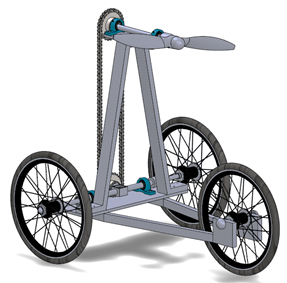
\includegraphics[width=\linewidth]{images/part9/drivetrainIter1.png}
%     \caption{Vehicle Iteration 1}
%     \label{fig:dtIter11}
% \end{wrapfigure}

\begin{figure}[!htbp]
    \centering
    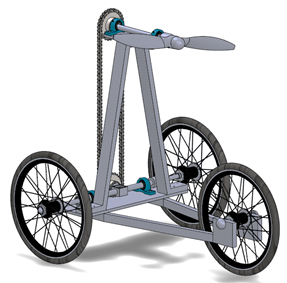
\includegraphics{images/part9/drivetrainIter1.png}
    \caption{Vehicle Iteration 1}
    \label{fig:dtIter1}
\end{figure}

In this iteration, the wheel choice, sprocket size choice, and propeller design were completed, along with the chain tensioner mechanism design. The axle was positioned underneath the bottom plate, to allow the structural members to be easily attached above via bolts. The chain tensioner allows tension to be applied to the chain during testing to prevent it from derailing. The propeller and the chain drive are situated on either side of the A-frame, which provides solid support via two pillow block bearings. Connections for the wheels were finalised to utilize the existing hubs on the wheels, with the front wheel being mounted via a small front fork manufactured from 6 mm aluminium plates, fixed onto the existing front axle. The rear wheels were mounted to the axle threaded at both sides, by nuts clamping the existing hubs (bearings removed) to the axle, locking the rotation.

Making the strut beams modular whilst achieving sufficient structural rigidity meant that the beams could not be directly welded onto the rear base plate that held the rear axle in place. To achieve this, a set of aluminium brackets were made by cutting sheet metal using a water jet cutter and welding them together at the specific angle required. The bottom brackets were made from 4 mm aluminium and the top bracket with 3mm aluminium. To supplement the brackets, a pair of aluminium blocks made with a CNC were made. These would be bolted together with the sheet metal brackets and help support the 20x40mm aluminium bars in compression load on each side. The design of these blocks were kept simple with minimal curvature to decrease the time of manufacture. During the assembly process, however, it was found that the sheet metal brackets were sufficiently strong to hold loads and therefore it was decided to not use them for testing.

A new iteration of the design was manufactured successfully for the preliminary wind tunnel test. During the test without the propeller attached, it experienced resonance due to non-concentric wheels causing a forced vibration which caused the A-frame to resonate, as explained in the "Resonance analysis" section. The problems due to this were addressed in iteration three of the design, where minor changes were made to the vehicle design before the 2nd wind tunnel test.

\begin{figure}[!htbp]
    \centering
    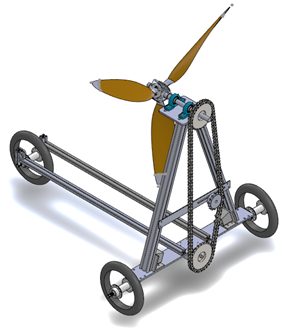
\includegraphics{images/part9/drivetrainIter2.png}
    \caption{Vehicle Iteration 2}
    \label{fig:dtIter2}
\end{figure}

Iteration 3 implements the design changes due to the resonance found in the initial testing of the vehicle. From combined analyses of test footage and simulations through the finite element analysis shown in the following section, it was found that fixing the propeller mount to the front wheel would likely decrease oscillations. It was decided that a strut must be placed between the top of the A-frame and the front wheel. This was done by adding an extra 20x20 mm strut member and this was connected using a separate set of custom brackets similar to the ones used to connect the A-frame to the rear base plate and top propeller mount plate.

\begin{figure}[!htbp]
    \centering
    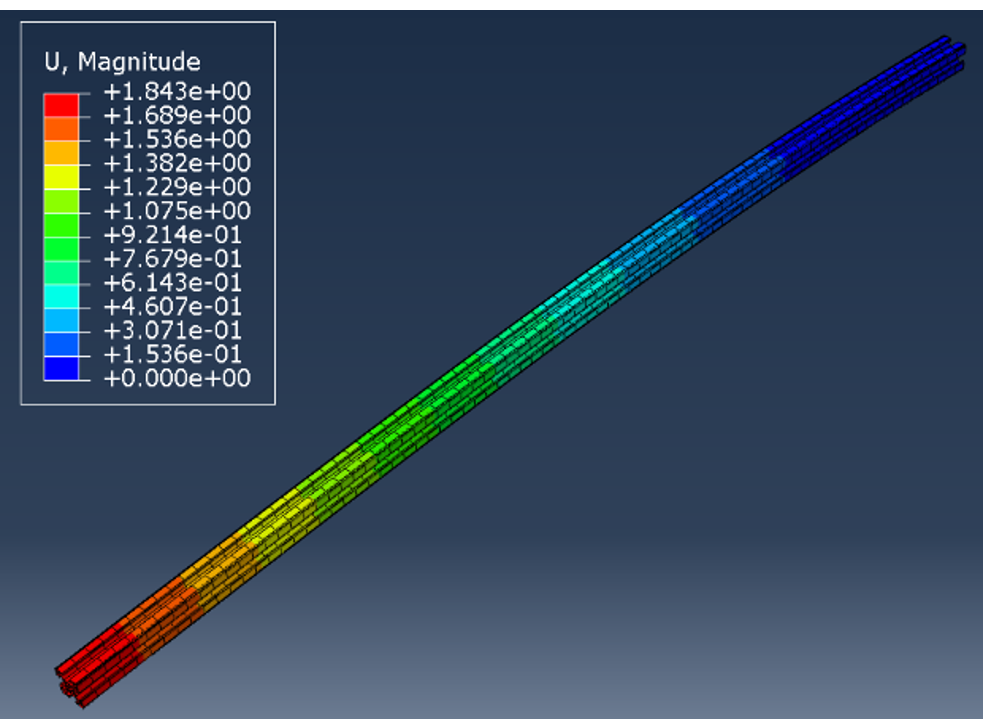
\includegraphics[width=0.5\linewidth]{images/part8/stucturethingy.png}
    \caption{FEA simulation showing the deformation of an aluminium profile beam under a $5\mathbf{kN}$ concentrated load}
    \label{fig:structhingy}
\end{figure}

\subsection{Manufacturing}
\begin{table}[!htbp]
    \centering
    \caption{Material properties}
    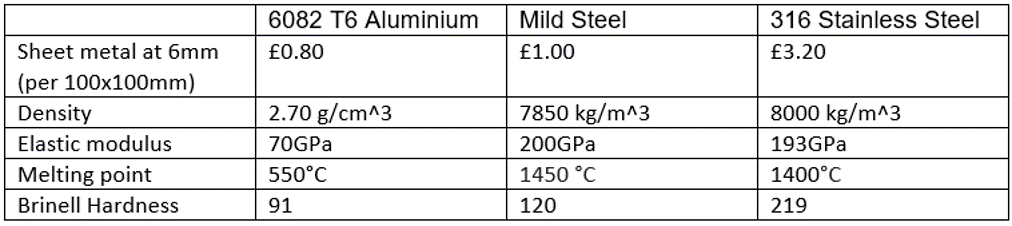
\includegraphics[width = \linewidth]{images/part8/materials.png}
    \label{tab:materials}
\end{table}

Table \ref{tab:materials} displays the generic material properties of the three sheet metals available in the EDMC. Within the project it was important to keep within the budget, therefore the main factor for this decision was the cost of the material. For the 6mm plate, the aluminium was the cheapest option and had the benefit of the lowest density and therefore weight. It was understood that the metal had a lower elastic modulus and hardness, but reducing the costs and weight were the main priorities, leading us to a decision of Aluminium.

The profile of the bar that was used in the experiment depended on two main factors: the deformation and the availability. Simple FEA analysis was conducted into the deformation characteristics of all the bar profiles, taking note of second moments of area and applying a uniform load. The FEA model was conducted under a simple Eulerian format which would induce the simplest deformation. The simple linear elastic model was applied in ABACUS and was applied to a model with the same length.


From the table of results, it’s clear that the I beam performs the best out of all the different beams when a point load is applied at one end. This demonstrates how this beam has the best directionality vertically than the other beams. The square beam also performs relatively well when tasked with deformation and has the benefit of having multiple directions of stability. The aluminium profile bar was modelled differently from the other bar types due to the complex nature of the bar profile. Inputting a DXF file into ABACUS I modelled the bar as a solid profile and deformed the structure. The deformation values were higher for the aluminium profile beam, but this was due to the limited computational cost availability. With more cell accuracy the deformation would drop significantly and gain a value much more similar to the I beam than is seen. With the aluminium profile, there are specific companies specialising in providing metal services. Bars can be pre-cut to specific lengths and less pressure will be put on connecting as the bars can be connected through the brackets that are also available on the websites. To increase the modularity of the vehicle, the best option would be to go for the aluminium profile to increase the modularity of the vehicle and project.

\subsection{Resonance analysis}

Before the completion of the vehicle, several wind tunnel tests were run without the propeller. This was useful in gauging approximate efficiencies of the wheels, gearbox, and drivetrain. As part of these tests, the moving ground was run between 0-10 m/s. It was observed that at around 3.5 m/s a resonance was set up in the A-frame (5.5 Hz) that yielded the vehicle very unstable to the point that a partial redesign would be necessary. The primary source of the energy input appeared to be the wheels which produced a driving frequency of twice their revolutions per second. This led to deriving a moving ground velocity – natural frequency relationship that would help to improve the vehicle’s stability:

\begin{equation}
V=\frac{f_{n} \times \pi D_{w h e e l}}{2} \approx 0.64 f_{n} m
\label{eq:natfreq}
\end{equation}

Thus, by increasing the natural frequency of the A-frame, which is effectively an inverted pendulum, the moving ground velocity for resonance to occur can be strategically placed much higher than the tested. A second improvement would be a stiffened A-frame that would oscillate with much lower amplitudes during resonance.

For validation, subsequent studies were made using SolidWorks frequency analysis using a simplified model of the vehicle shown in Figure \ref{fig:freqStudy}, where red regions represent the areas of highest deflection. The results showed that its mode 1 resonant frequency was 6.48 Hz (Corresponding to a rolling road speed of 4.14 m/s). This is slightly higher than observed in the wind tunnel but is likely down to real-world damping from unmodelled vehicle components. It is however similar enough for further testing.

\begin{figure}[!htbp]
    \centering
    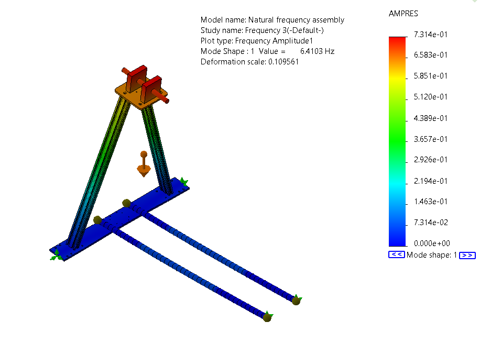
\includegraphics{images/part8/freqStudy.png}
    \caption{SolidWorks frequency study of vehicle}
    \label{fig:freqStudy}
\end{figure}

Three potential modifications were tested to assess their impact on the natural frequency of the vehicle:

\begin{itemize}
  \item A cross-beam structural member connecting top of A-frame to front of vehicle
  \item Larger plate at base of vehicle
  \item Thicker chassis members (increase second moment of area)
\end{itemize}

Performing SolidWorks frequency analysis on these variations (Figure \ref{fig:freqStudy2}) found that the latter two options did not sufficiently increase the natural frequency of the A-frame (12.2 Hz and 7.8 Hz respectively). Whilst their relative deflections were smaller, they do not entirely solve the problem of pushing resonance away from the operating speeds of the vehicle in the wind tunnel. The cross-beam option however was very effective, placing the natural frequency at around 76.8 Hz corresponding to a rolling road speed of 49.2 m/s. This design change would be critical but require moving the prop from the front of the A-frame to the back.

\begin{figure}[!htbp]
    \centering
    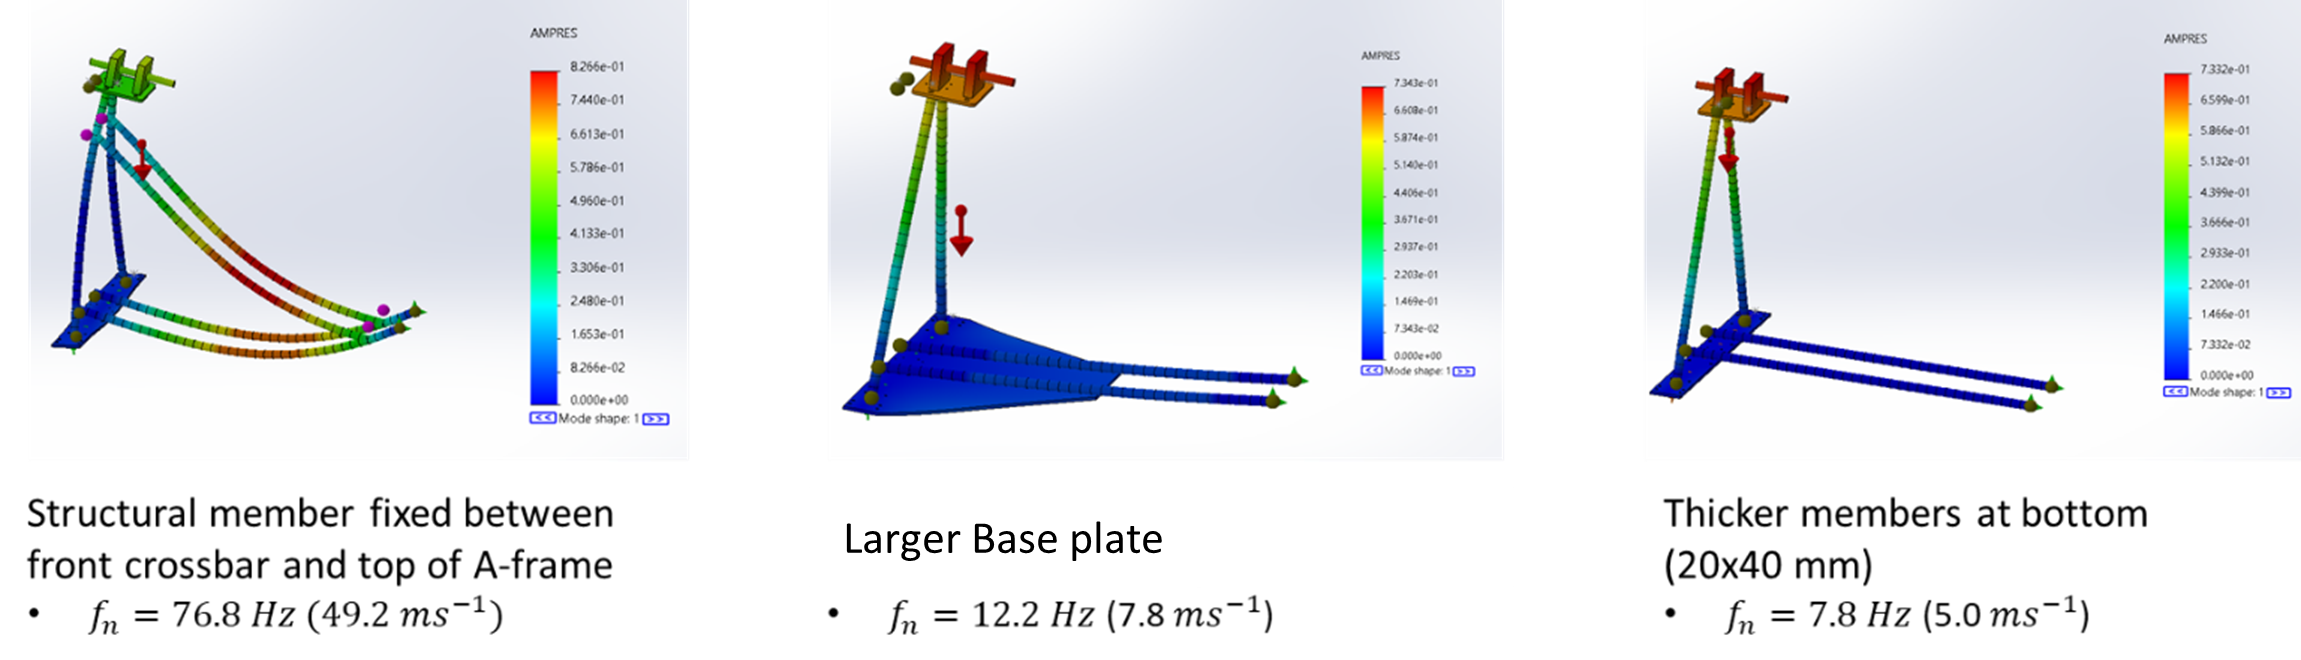
\includegraphics{images/part8/freqStudy2.png}
    \caption{Frequncy study of vehicle improvements}
    \label{fig:freqStudy2}
\end{figure}

\subsection{Structural update and vehicle reconfiguration}

This updated design takes into account the changes made due to the problems mentioned in the above section. To solve this, a 20x20 aluminium profile was fixed between the top of the A-frame and the front crossbar, and represents iteration three of the structure. This meant that the chain drive, propeller, and chain tensioner needed to be mirrored about the A-frame, which was a simple task due to the symmetry of the design. This allowed sufficient space for the supporting profile to be fitted effectively. It also meant that the propeller operated in a pusher configuration. The implications of this reconfiguration on propeller efficiency was not assessed further as the flow would likely be minimally affected by the this change.

\begin{figure}[!htbp]
    \centering
    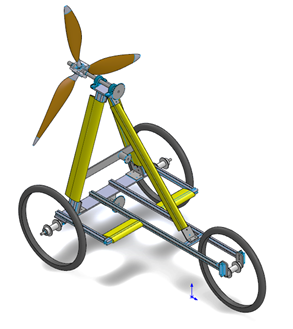
\includegraphics{images/part9/drivetrainIter3.png}
    \caption{Vehicle Iteration 3}
    \label{fig:dtIter3}
\end{figure}

\subsection{Aerodynamic streamlining}

Due to the jagged geometry of the aluminium extrusions used for the structure, an attempt was made to partially streamline the members ahead of the propeller for a potential improvement in performance. The design for this was made using a NACA 0030 aerofoil cross-section (The largest thickness to chord ratio plottable) wrapped around each beam. Two variations were made for the 20x20  mm and 20x40 mm bars (Figure \ref{fig:fairing3}), extending the 'width' of the beams by a mere 3 mm and 5 mm respectively. 3D printing was once again the go to option for manufacture, as the geometries could be produced quickly. Due to the lack of strength required for these parts, they could be printed using a single wall and no infill, and with the inclusion of a slot in the trailing edge could be opened and placed around the bar. These fairings were placed on several beams ahead of the propeller, however, time constraints and an increased focus on propeller manufacture meant that not all sections could be covered.

\begin{figure}[!htbp]
    \centering
    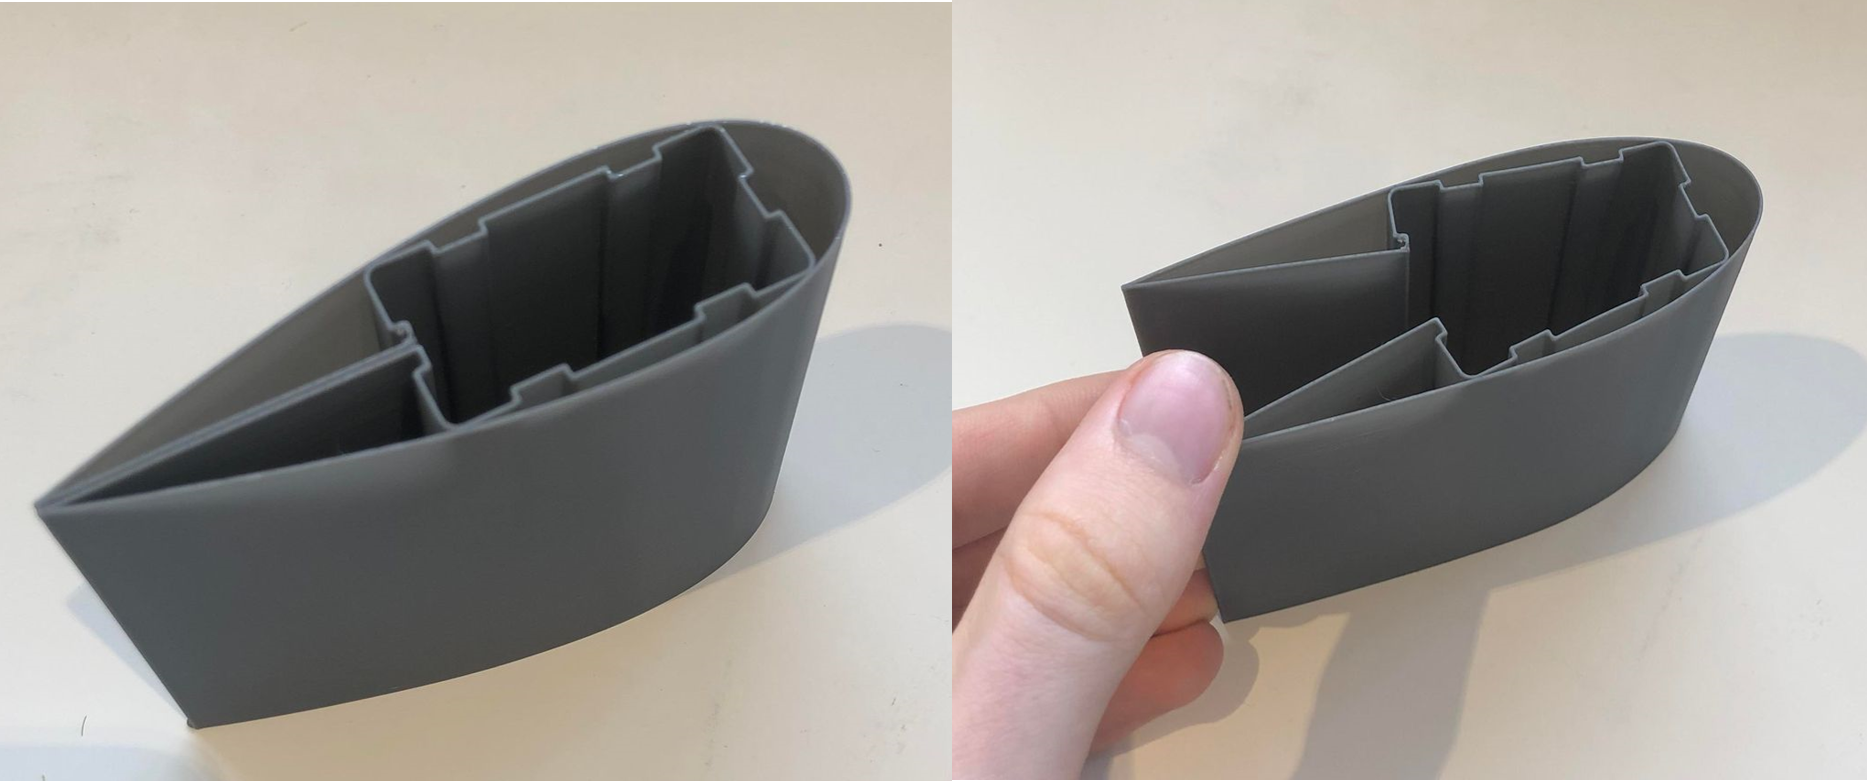
\includegraphics{images/part8/fairing3.png}
    \caption{3D printed fairing for aluminium extrusions}
    \label{fig:fairing3}
\end{figure}
